%%
%% This is file `sample-sigchi.tex',
%% generated with the docstrip utility.
%%
%% The original source files were:
%%
%% samples.dtx  (with options: `sigchi')
%% 
%% IMPORTANT NOTICE:
%% 
%% For the copyright see the source file.
%% 
%% Any modified versions of this file must be renamed
%% with new filenames distinct from sample-sigchi.tex.
%% 
%% For distribution of the original source see the terms
%% for copying and modification in the file samples.dtx.
%% 
%% This generated file may be distributed as long as the
%% original source files, as listed above, are part of the
%% same distribution. (The sources need not necessarily be
%% in the same archive or directory.)
%%
%% The first command in your LaTeX source must be the \documentclass command.
\documentclass[sigchi]{acmart}

%%
%% \BibTeX command to typeset BibTeX logo in the docs
% \AtBeginDocument{%
%   \providecommand\BibTeX{{%
%     \normalfont B\kern-0.5em{\scshape i\kern-0.25em b}\kern-0.8em\TeX}}}
\AtBeginDocument{%
  \providecommand\BibTeX{{%
    \normalfont B\kern-0.5em{\scshape i\kern-0.25em b}\kern-0.8em\TeX}}}

\settopmatter{printacmref=false} % Removes citation information below abstract
\renewcommand\footnotetextcopyrightpermission[1]{} % removes footnote with conference information in first column
\pagestyle{plain} % removes running headers
\usepackage{caption}
\usepackage{svg}
\usepackage{graphics}
\usepackage{amsmath}
\usepackage[british]{babel}
\usepackage{xcolor}
\usepackage{CJKutf8}
% \usepackage{cite}
% \usepackage{graphicx}
\usepackage{subcaption}
\usepackage{listings}
\usepackage{color}
% \usepackage{graphicx}
\usepackage{subcaption}
\definecolor{dkgreen}{rgb}{0,0.6,0}
\definecolor{gray}{rgb}{0.5,0.5,0.5}
\definecolor{mauve}{rgb}{0.58,0,0.82}

\lstset{frame=tb,
  language=C,
  aboveskip=3mm,
  belowskip=3mm,
  showstringspaces=false,
  columns=flexible,
  basicstyle={\small\ttfamily},
  numbers=none,
  numberstyle=\tiny\color{gray},
  keywordstyle=\color{blue},
  commentstyle=\color{dkgreen},
  stringstyle=\color{mauve},
  breaklines=true,
  breakatwhitespace=true,
  tabsize=3
}
%% Rights management information.  This information is sent to you
%% when you complete the rights form.  These commands have SAMPLE
%% values in them; it is your responsibility as an author to replace
%% the commands and values with those provided to you when you
%% complete the rights form.
% \setcopyright{}
% \copyrightyear{}
% \acmYear{}
% \acmDOI{}

%% These commands are for a PROCEEDINGS abstract or paper.
% \acmConference[Woodstock '18]{Woodstock '18: ACM Symposium on Neural
%   Gaze Detection}{June 03--05, 2018}{Woodstock, NY}
% \acmBooktitle{Woodstock '18: ACM Symposium on Neural Gaze Detection,
%   June 03--05, 2018, Woodstock, NY}
% \acmPrice{15.00}
% \acmISBN{978-1-4503-9999-9/18/06}


%%
%% Submission ID.
%% Use this when submitting an article to a sponsored event. You'll
%% receive a unique submission ID from the organizers
%% of the event, and this ID should be used as the parameter to this command.
%%\acmSubmissionID{123-A56-BU3}

%%
%% The majority of ACM publications use numbered citations and
%% references.  The command \citestyle{authoryear} switches to the
%% "author year" style.
%%
%% If you are preparing content for an event
%% sponsored by ACM SIGGRAPH, you must use the "author year" style of
%% citations and references.
%% Uncommenting
%% the next command will enable that style.
%%\citestyle{acmauthoryear}

%%
%% end of the preamble, start of the body of the document source.
\begin{document}

%%
%% The "title" command has an optional parameter,
%% allowing the author to define a "short title" to be used in page headers.
\title{Master thesis proposal \\
       A container based self-adjusted auto-provisioning framework 
        at resource level}

%%
%% The "author" command and its associated commands are used to define
%% the authors and their affiliations.
%% Of note is the shared affiliation of the first two authors, and the
%% "authornote" and "authornotemark" commands
%% used to denote shared contribution to the research.
\author{You Hu}
\email{adolphus.hu@student.vu.nl}
\affiliation{%
  \institution{VU Amsterdam }
%   \city{Amsterdam}
}



%%
%% By default, the full list of authors will be used in the page
%% headers. Often, this list is too long, and will overlap
%% other information printed in the page headers. This command allows
%% the author to define a more concise list
%% of authors' names for this purpose.
\renewcommand{\shortauthors}{You Hu}

%%
%% The abstract is a short summary of the work to be presented in the
%% article.



%%
%% Keywords. The author(s) should pick words that accurately describe
%% the work being presented. Separate the keywords with commas.


%%
%% This command processes the author and affiliation and title
%% information and builds the first part of the formatted document.
\maketitle

\section{Introduction}
The Netherlands eScience Center has developed solutions for calibrating imaged observation collected by LOw Frequency Array(LOFAR) telescope\footnote{\url{http://www.lofar.org/}}.
The LOFAR consists of 51 stations cross Europe and a typical LOFAR observation has the size of 100TB, after friquency averaing, the size can be reduced to 16TB. \cite{Spreeuw2019}
Collectively, there are over 5 PB of data will be stored each year. \cite{Start2020} To calibrate the observation by given sky map, SAGECaL is invented and implemented for this purpose.\cite{Kazemi2011}
By given pre-processed observation data, sky model and parameters, the calibration can be done independently. However, it is a compuation comsuming application. Currently, eScience Center has developed GPU, MPI and Spark versions for acceleration.
All of them have achieved great acceleration compared to the naive version. 

However, the solutions following horizontal scaling idea, MPI and Spark, will lead to a waste of computation resources in non-dedicated clusters.
In this project, we try to build up a system to achive auto provisioning at public clusters to drive the computation consuming applications. This solution can be applied to other more applications with the demond of auto-provisioning.

\section{The common issue on current versions}
Both MPI version\footnote{\url{https://github.com/nlesc-dirac/sagecal/tree/master/src/MPI}} and Spark version\footnote{\url{https://github.com/nlesc-dirac/sagecal-on-spark}} take SAGECaL process as a black box, it aims to schedule the task on multiple nodes to achieve acceleration. 
For MPI version, the architecture is master-worker like, but the task scheduling mechanism is very simple. In Spark version, the tasks are carried by driver with Java Native Interface. And each task is invoking encapsulated C++ program.
The common issue of MPI and Spark version is that the resources can be not be fully utilized in non-dedicated cluster. 

\begin{figure}[h!]
  \begin{subfigure}[b]{0.45\textwidth}
      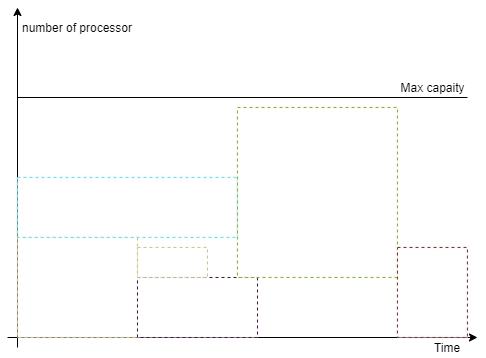
\includegraphics[width=\textwidth]{img/MPI_batch.png}
      \caption{Resources utilization of MPI batch jobs on cluster}
      \label{fig:MPI_batch}
  \end{subfigure}
  \begin{subfigure}[b]{0.45\textwidth}
      
\includegraphics[width=\textwidth]{img/spark_NP.png}
      \caption{Resources utilization of Spark on cluster}
      \label{fig:spark_np}
  \end{subfigure}
  \caption{The waste of compuation on cluster}\label{fig:waste_cluster}
\end{figure}
The resource utilization of these two systems can be visualized as Fig. \ref{fig:waste_cluster}. As it is shown in Fig. \ref{fig:MPI_batch}, MPI jobs are scheduled as fixed batch jobs which are colored boxes in the figure. It is very common to meet the situation that all jobs in the queue are too large and the number of idle resources is not enough for the jobs in the queue. 
For Spark version, the possible situation can be visualized as Fig. \ref{sub@fig:spark_np}. The nodes should be reserved for Spark in advance and Spark handles the task scheduling. For typical Spark applications relying on RDD, the number of required executors can be up and down dynamically. Part of computation resources may be wasted since this computation power is exclusive for Spark.
However, of course, the current Spark implementation for calibration is based on Driver mode and the granularity is one executor per task. In this case, the waste of resources won't happen within the Spark cluster. But when there are a lot of idle nodes in the cluster that not reserved for Spark at the beginning, they can not be used for Spark. 


\section{Research question statement}
 
\newpage
\bibliography{sample-base.bib}
\bibliographystyle{ACM-Reference-Format}

\end{document}
\endinput
%%
%% End of file `sample-sigchi.tex'.
